\documentclass[aspectratio=169,10pt]{beamer}
\usepackage[utf8]{inputenc}
\usepackage[T1]{fontenc}
\usepackage{lmodern}
\usepackage{booktabs}
\usepackage{graphicx}
\usepackage{xcolor}

\usetheme{Madrid}
\definecolor{unilublue}{RGB}{15,44,89}
\definecolor{tealaccent}{RGB}{15,118,110}
\setbeamercolor{structure}{fg=unilublue}
\setbeamercolor{title}{bg=unilublue,fg=white}
\setbeamercolor{frametitle}{bg=unilublue,fg=white}
\setbeamertemplate{navigation symbols}{}

\title[Projet Final --- Syst\`emes UNIX]{Analyse de Donn\'ees avec Pipeline UNIX}
\subtitle{D\'eploiement, Traitement, Visualisation et Reporting}
\author[Lutumba Miteo Eric]{Lutumba Miteo Eric \\ \scriptsize Enseignant : Prof. Patrick Mukala}
\institute[UNILU --- M1 Info]{Universit\'e de Lubumbashi \\ Facult\'e des Sciences --- D\'epartement d'Informatique (M1)}
\date{D\'ecembre 2026}

\begin{document}

\begin{frame}
    \titlepage
\end{frame}

\begin{frame}{1. Contexte, Cahier des Charges et Deux Modes de Simulation}
    \begin{itemize}
        \item \textbf{9 villes fran\c{c}aises impos\'ees} : Paris, Lyon, Marseille, Lille, Bordeaux, Toulouse, Nantes, Nice, Strasbourg sur 3 mois.
        \item \textbf{Mode EXAM (\texttt{MODE=exam}, d\'efaut)} : 2\,500 livraisons de base (2\,555 brutes), 35 livreurs, 1\,200 logs HTTP Apache.
        \item \textbf{Mode EXTENDED (\texttt{MODE=extended})} : 12\,000 livraisons/mois/ville ($\sim$330\,000 lignes sur 3 mois) avec coefficients de march\'e et saisonnalit\'e configurables.
    \end{itemize}
\end{frame}

\begin{frame}{2. Architecture Conteneuris\'ee (Docker + Traefik + PostgreSQL + Metabase)}
    \begin{columns}[T]
        \begin{column}{0.52\textwidth}
            \textbf{4 services avec \texttt{healthcheck} :}
            \begin{enumerate}
                \item \textbf{\texttt{traefik}} (\texttt{v3.2}) : reverse proxy unique (\texttt{metabase.localhost:8080}).
                \item \textbf{\texttt{dev}} (Debian / Python 3.14, non-root UID 1000) : filtres UNIX, \texttt{gnuplot}, \texttt{shellcheck}, \texttt{iragi}.
                \item \textbf{\texttt{db}} (PostgreSQL 16) : \texttt{couriers}, \texttt{deliveries}, \texttt{web\_access\_logs}.
                \item \textbf{\texttt{dashboard}} (Metabase) : BI connect\'ee \`a PostgreSQL.
            \end{enumerate}
        \end{column}
        \begin{column}{0.46\textwidth}
            \textbf{Commandes exactes :}
            \begin{itemize}
                \item \texttt{./bin/launch.sh}
                \item \texttt{make generate-data MODE=exam}
                \item \texttt{make pipeline}
                \item \texttt{make load-db}
                \item \texttt{./bin/test.sh}
                \item \texttt{./bin/backup.sh}
            \end{itemize}
        \end{column}
    \end{columns}
\end{frame}

\begin{frame}{3. Pipelines UNIX et R\^ole Scientifique d'\texttt{iragi} (\texttt{v0.6.4})}
    \begin{table}
        \centering
        \scriptsize
        \begin{tabular}{lccc}
            \toprule
            \textbf{Crit\`ere} & \textbf{1. Brut (\texttt{raw})} & \textbf{2. Classique na\"if} & \textbf{3. UNIX + \texttt{iragi}} \\
            \midrule
            Lignes retenues & 2\,555 & 2\,520 & \textbf{2\,510 (parit\'e exacte)} \\
            Doublons actifs & 35 & 0 & \textbf{0} \\
            Violations \texttt{DataContract} & 12 & \textcolor{red}{\textbf{10 actives}} & \textcolor{tealaccent}{\textbf{0 (100 \% filtr\'ees)}} \\
            Quarantaine DLQ & 0 & Aucune & \textcolor{tealaccent}{\textbf{10 lignes isol\'ees}} \\
            Orphelins HTTP \texttt{404} & 139 ignor\'es & 139 ignor\'es & \textcolor{tealaccent}{\textbf{139 identifi\'es (\texttt{reconcile})}} \\
            Score \texttt{iragi.scan} & 99,29 / 100 & Non certifi\'e & \textcolor{tealaccent}{\textbf{99,75 / 100 (+0,46 pt)}} \\
            \bottomrule
        \end{tabular}
    \end{table}
\end{frame}

\begin{frame}{4. Comparaison des Anomalies : Brut vs Classique vs UNIX + \texttt{iragi}}
    \centering
    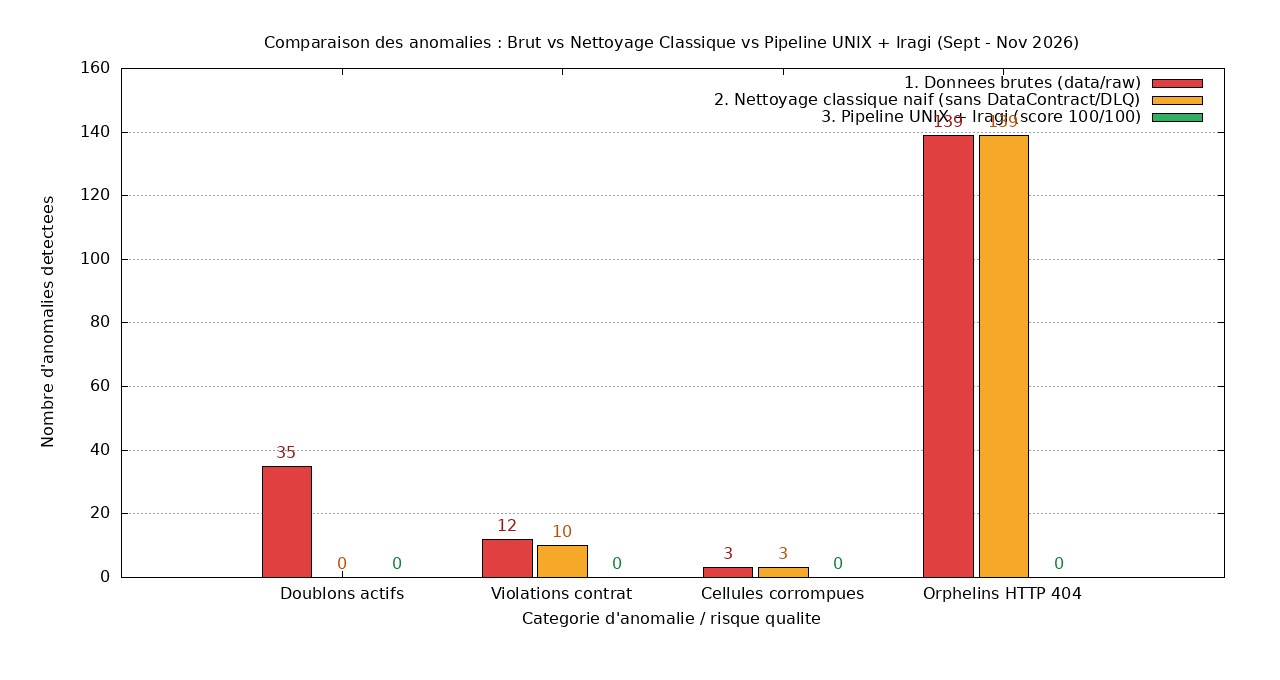
\includegraphics[height=0.76\textheight]{../data/visualizations/08_anomalies_avant_apres.png}
\end{frame}

\begin{frame}{5. Volume et Taux de Retard par Ville (Mode EXAM)}
    \begin{columns}[T]
        \begin{column}{0.49\textwidth}
            \centering
            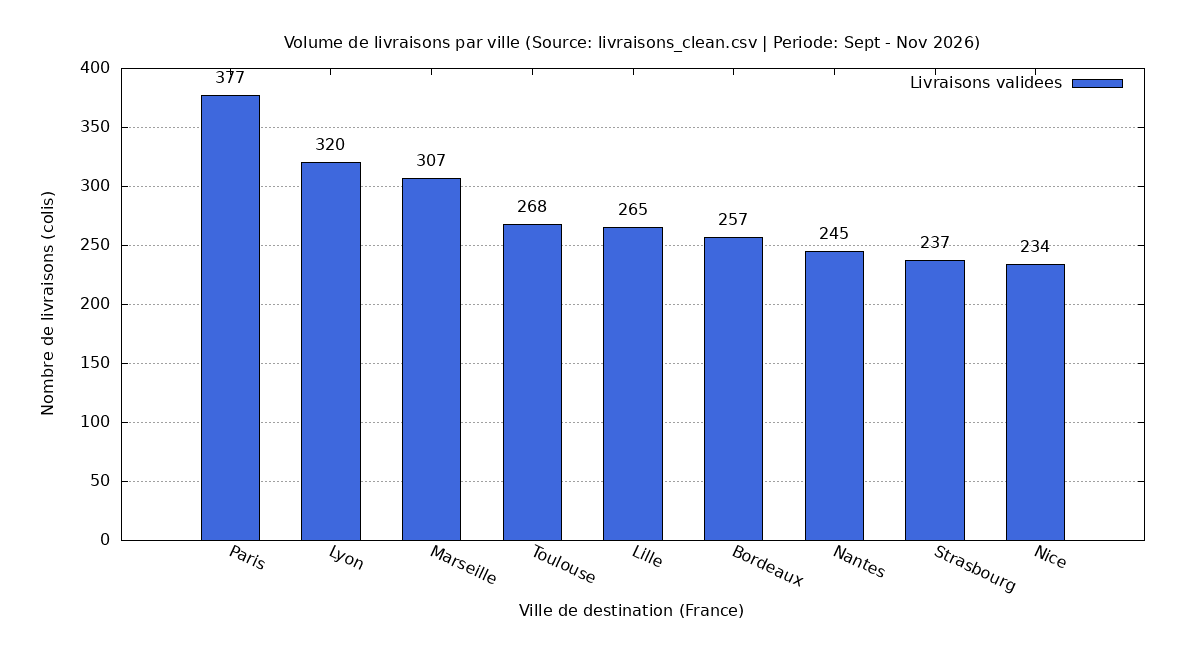
\includegraphics[width=\textwidth]{../data/visualizations/01_livraisons_par_ville.png}
        \end{column}
        \begin{column}{0.49\textwidth}
            \centering
            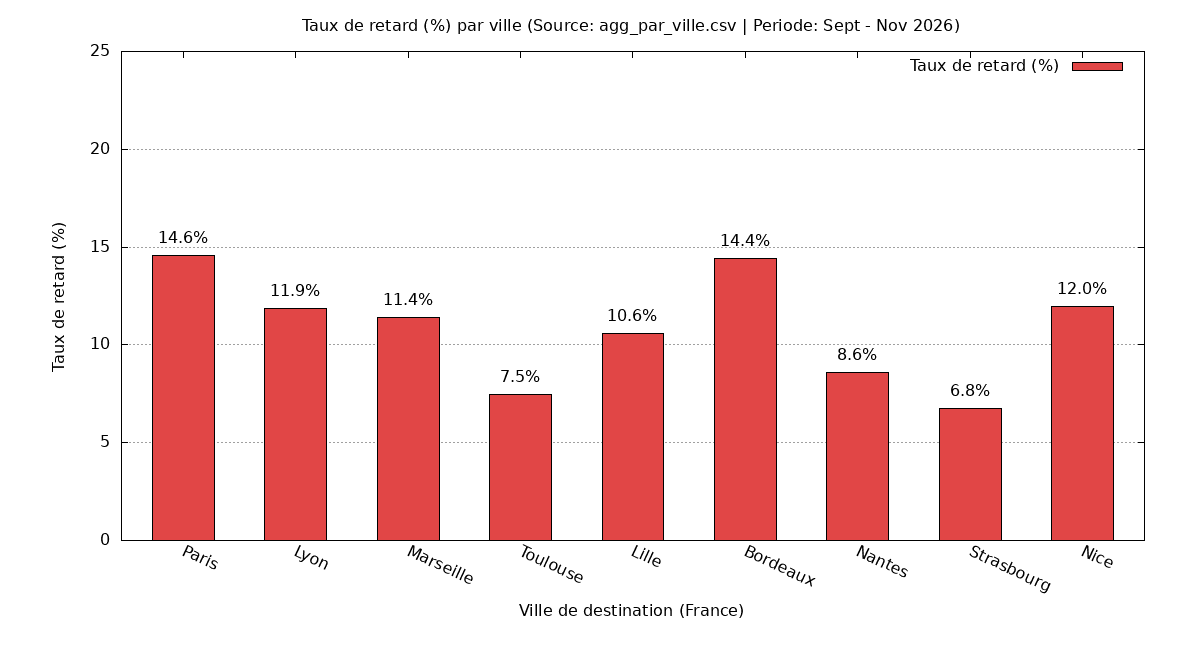
\includegraphics[width=\textwidth]{../data/visualizations/03_taux_retard_par_ville.png}
        \end{column}
    \end{columns}
\end{frame}

\begin{frame}{6. Corr\'elation Distance/Temps ($r = 0,9296$) et Distribution des Dur\'ees}
    \begin{columns}[T]
        \begin{column}{0.49\textwidth}
            \centering
            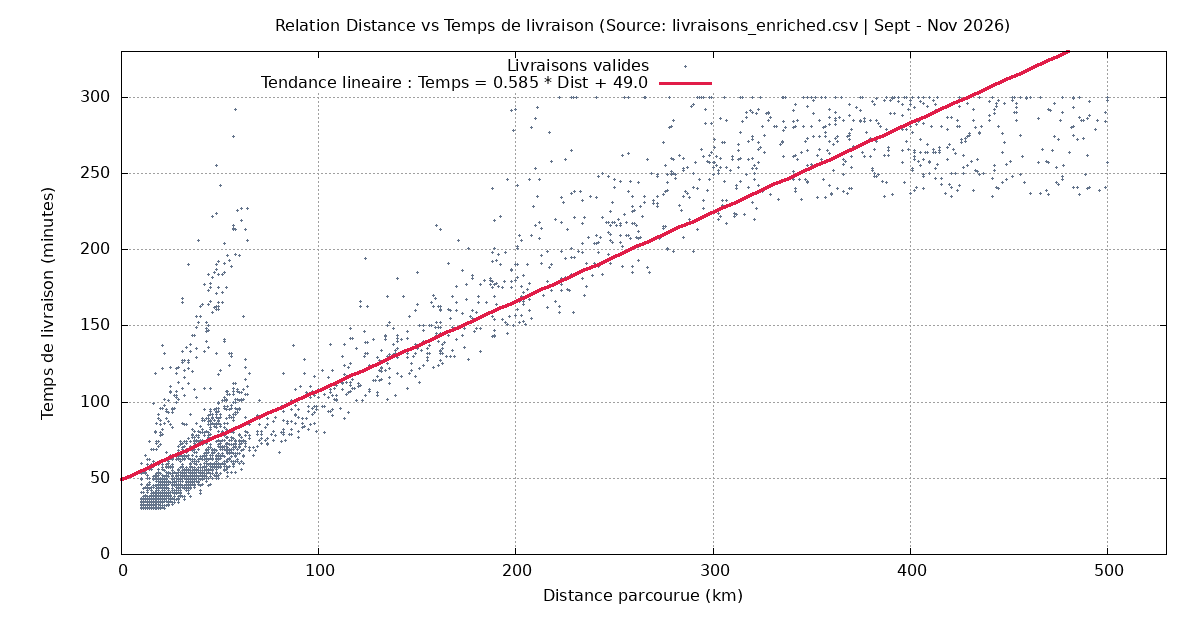
\includegraphics[width=\textwidth]{../data/visualizations/05_distance_vs_temps.png}
        \end{column}
        \begin{column}{0.49\textwidth}
            \centering
            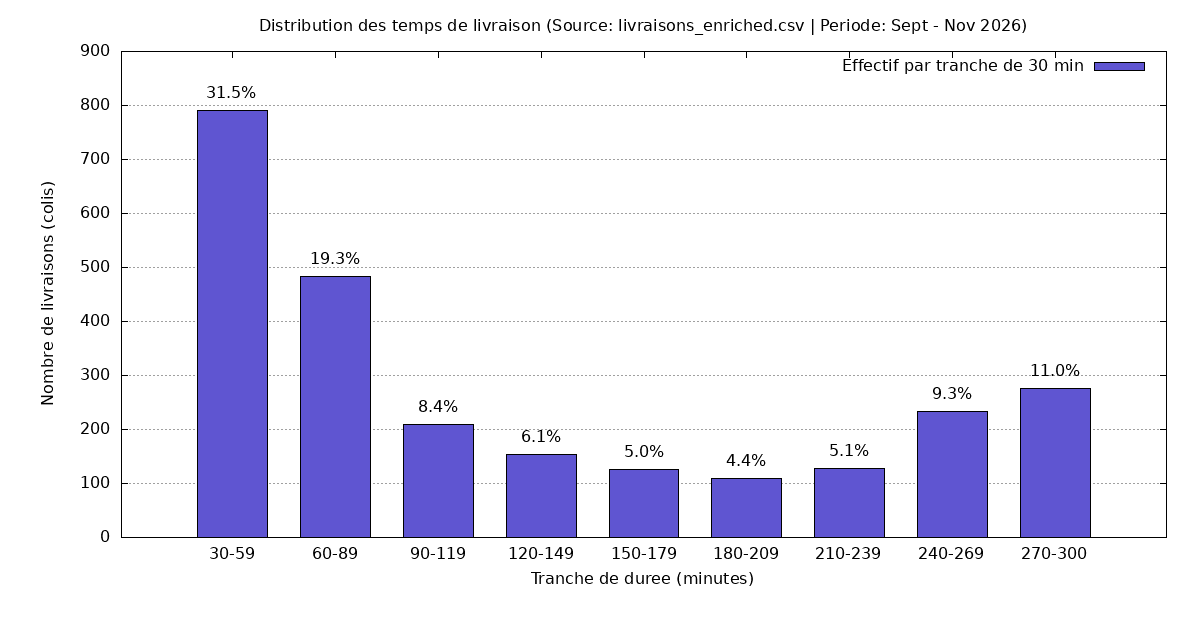
\includegraphics[width=\textwidth]{../data/visualizations/04_distribution_temps.png}
        \end{column}
    \end{columns}
\end{frame}

\begin{frame}{7. Validation Bout-en-Bout, Mode EXTENDED et Conclusion}
    \begin{itemize}
        \item \textbf{PostgreSQL + Metabase} : chargement v\'erifi\'e de 35 livreurs, 2\,510 livraisons et 1\,200 logs HTTP ; Metabase sain derri\`ere Traefik (\texttt{http://metabase.localhost:8080}).
        \item \textbf{Mont\'ee en charge (\texttt{MODE=extended})} : 329\,410 livraisons propres trait\'ees en 21 secondes avec bascule automatique sur \texttt{iragi.scan\_csv\_stream}.
        \item \textbf{Qualit\'e} : \textbf{17/17 tests TDD pass\'es}, \textbf{0 alerte \texttt{shellcheck}}, documentation Sphinx et sauvegardes SHA-256.
    \end{itemize}
\end{frame}

\end{document}
